%----------------------------------------------------------------------------------------
%	PACKAGES AND DOCUMENT CONFIGURATIONS
%----------------------------------------------------------------------------------------

\documentclass{article}

\usepackage[version=3]{mhchem} % Package for chemical equation typesetting
\usepackage{siunitx} % Provides the \SI{}{} and \si{} command for typesetting SI units
\usepackage{graphicx} % Required for the inclusion of images
\usepackage{natbib} % Required to change bibliography style to APA
\usepackage{amsmath} % Required for some math elements 
\usepackage{amssymb}
\graphicspath{ {./images/} }


\setlength\parindent{0pt} % Removes all indentation from paragraphs

\renewcommand{\labelenumi}{\alph{enumi}.} % Make numbering in the enumerate environment by letter rather than number (e.g. section 6)

%\usepackage{times} % Uncomment to use the Times New Roman font

%----------------------------------------------------------------------------------------
%	DOCUMENT INFORMATION
%----------------------------------------------------------------------------------------

\title{ASSIGNMENT 1: Fast Trajectory Planning} % Title, replace [N] with the current week number

\author{ERICA CAI, BONING DING, and SHREYA JAHAGIRDAR} % Author name

\date{\today} % Date for the report

\begin{document}

\maketitle % Insert the title, author and date

\begin{center}
\begin{tabular}{l r}
Professor: & Abdeslam Boularias \\ % Partner names
Teaching Assistants: & Aravind Sivaramakrishnan  \\ 
&  Yuting Wang \\ % remove names if not needed, TO GET more copy this line exactly
& Yikai Zhang \\

Introduction to Artificial Intelligence \\
Rutgers University, New Brunswick  \\
\end{tabular}
\end{center}

%----------------------------------------------------------------------------------------
%	SECTION 1
%----------------------------------------------------------------------------------------

\section{Part 0 - Set Up Environments}

x
%----------------------------------------------------------------------------------------
%	SECTION 2
%----------------------------------------------------------------------------------------

\section{Part 1 - Understanding the Methods}

\subsection{Explain in your report why the first move of the agent for the example search problem from Figure 8 is to the east rather
than the north given that the agent does not know initially which cells are blocked.}

\begin{figure}[h!]
  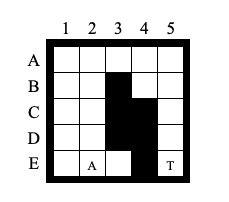
\includegraphics[width=0.5\textwidth]{p1_0.png}
  \caption{The actual grid }
\end{figure}

By definition, A* search will return the shortest path from A to T.\\

Initially, the agent does not know that any cells are blocked. Although the actual grid is shown in Figure 1, the agent perceives the grid to be as shown in Figure 2.  \\

\begin{figure}[h!]
  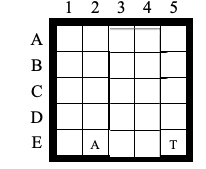
\includegraphics[]{p1_1.png}
  \caption{The agent's perspective of the grid }
\end{figure}

In this grid shown in Figure 2, the shortest path from  A to T is E2, E3, E4, E5. There is no path from A to T that is shorter. Since A* search returns the shortest path, A* search will return the path E2, E3, E4, E5.\\

Believing that Figure 2 is the grid, the agent will move along this path, first moving to the east, to E3. \\

We know that in the actual grid shown in Figure 1, the shortest path from A to T involves moving to the north first, to circumvent the obstacles, to get to T. However, the agent does not know that these obstacles exist. As a result, the agent will move to the east, believing that it is following a shorter path. \\

\subsection{Give a convincing argument that the agent in finite gridworlds indeed either reaches the target or discovers that this is impossible in finite time. }
We want to show 1. That the agent reaches the target in finite time, and 2. That the agent discovers that reaching the target is impossible in finite time. \\\\
1. Show that the agent reaches the target in finite time.
\begin{enumerate}
	\item If there is a path from the start state to the goal, then, if there is a path from the start state to state x, that means there is a path from state x to the goal (because the agent can go from state x, back to the start state, and then to the goal). Therefore, if there is a path from the start state to the goal, and a path from the start state to state x, then A* search can ALWAYS find a path from the state x to the goal. 
	\item After many A* searches, the agent will know the grid environment and will be able to find an unblocked path from the state x to the goal. The number of A* searches is finite because the agent will always begin the A* search at a block where it has not begun an A* search before. This is because the agent already knows how to navigate the environment of any cell that it has started an A* search at before.
	\item Therefore, the agent reaches the target after a finite number of A* searches. Each A* search is finite, so the agent reaches the target in finite time.
\end{enumerate}
2. Show that the agent discovers that reaching the target is impossible in finite time.
\begin{enumerate}
	\item If there is no path from the start state to the goal, then, if there is a path from the start state to state x, that means there is no path from state x to the goal (because the agent can go from state x, and back to the start state, realizing that it cannot reach the goal).
	\item After many A* searches, the agent will know the grid environment and realize that there is no path from the state x to the goal. The number of A* searches is finite because the agent will always begin the A* search at a block where it has not begun an A* search before. This is because the agent already knows how to navigate the environment of any cell that it has started an A* search at before.
	\item Therefore, the agent realizes that reaching the target is impossible after a finite number of A* searches. Each A* search is finite, so the agent discovers that reaching the target is impossible in finite time.
\end{enumerate}

\subsection{Prove that the number of moves of the agent until it reaches the target or discovers that this is impossible is bounded from above by the number of unblocked cells squared.}

We want to show 1. That the number of moves of the agent until it reaches the target is bounded above by the number of unblocked cells squared  2. That the number of moves that the agent makes before discovering that reaching the target is impossible is bounded above by the number of unblocked squared.\\

In either case, 
\begin{enumerate}
	\item The agent makes at most the number of unblocked cells moves after each A* search. This is because, in the worst case, the agent will traverse every unblocked cell in the grid. 
	\begin{enumerate}
		\item Show that the A* search will never return a path that is longer than the number of unblocked cells.  If the number of moves is more than the number of unblocked cells, that means the path that the A* search returns is more than the number of unblocked cells. This means, the path includes a state (i,j) twice, according to the pigeonhole principle. Therefore, the path has a cycle. As a result, the path is not the shortest path; a shorter path exists which has no cycles. Since A* search always returns the shortest path, it will never return a path that is longer than the number of unblocked cells.
	\end{enumerate}
	\item The number of A* searches that the agent makes is at most the number of unblocked cells.
	\begin{enumerate}
		\item Show that the agent will always begin an A* search at a cell where it has not begun an A* search before.  The agent already knows how to navigate the environment of any cell that it has started an A* search at before. Therefore, it will not get blocked in a cell that it has started an A* search at before. As a result, it will not start an A* search at a cell that it has started at before. 
		\item Show that the number of A* searches that the agent makes cannot be more than the number of unblocked cells. The agent can only start a search at an unblocked cell. We know from part (a) that an agent will always begin an A* search where it has not begun an A* search before. Therefore, the agent must start the searchat  an unblocked cell that it has not started at before, and in the worst case, the agent will start the search the number of unblocked cells times.
	\end{enumerate} 
\end {enumerate}
We have just showed that the maximum number of moves that the agent can make is bounded by the number of unblocked cells squared. In part 2.2, we also showed that the agent reaches the target or discovers that this is impossible in finite time. Since the maximum number of moves is bounded by the number of unblocked cells squared, then the number of moves of the agent until it reaches the target or discovers that this is impossible is bounded from above by the number of unblocked cells squared.

%----------------------------------------------------------------------------------------
%	SECTION 3
%----------------------------------------------------------------------------------------

\section{Part 2 - The Effects of Ties}

\subsection{Implement and compare both versions of Repeated Forward A* with respect to their runtime or, equivalently, number of expanded cells.}
 
PUT TABLE HERE

\subsection{Explain your observations in detail, that is, explain what you observed and give a reason for the observation.}

Breaking ties in favor of cells with larger g-values is faster. Let two nodes, n and m, have the same f value. \\
According to the f value equation, we know

\[f_n = g_n + h_n \]
\[f_m = g_m + h_m \]

Assume that
\[f_n = f_m \]
\[g_n > g_m \]

Given these four equations, we know that
\[h_n<h_m\]

By definition, the h-value is an estimate of the distance between a node and the goal. Since node n has a smaller h-value than node m, then node n is closer to the goal than node m. Therefore, the agent is choosing to expand the node that is closer to the goal. \\
The node that is closer to the goal has a higher chance of being on the shortest path because there is a smaller distance to travel before reaching the goal.



%----------------------------------------------------------------------------------------
%	SECTION 4
%----------------------------------------------------------------------------------------

\section{Part 3 - Forward vs. Backward}

\subsection{Implement and compare Repeated Forward A* and Repeated Backward A* with respect to their runtime or, equivalently, number of expanded cells. }
PUT TABLE HERE
\subsection{Explain your observations in detail, that is, explain what you observed and give a reason for the observation.}
Repeated Forward A* will usually be faster than Repeated Backward A*. Let the agent perceive the grid to be as in Figure 3. In the grid, let A be the agent and T be the target.

\begin{figure}[h!]
  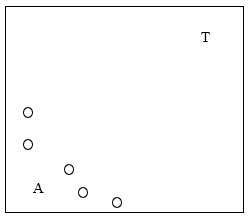
\includegraphics[width=0.5\textwidth]{p3_0.png}
  \caption{The agent's perception of the grid }
\end{figure}

The grid in Figure 3 is an accurate representation of an agent's perception of the grid because the agent knows the environment of cells that are close to it. However, the agent does not know the environment of cells that are far from it, such as for the cells that are close to T.

\begin{figure}[h!]
  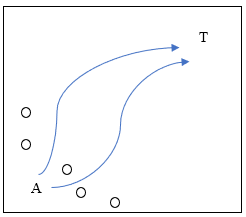
\includegraphics[width=0.5\textwidth]{p3_1.png}
  \caption{Possibilities for shortest paths from the agent to the target in Repeated Forward A*}
\end{figure}

The A* search in Repeated Forward A* will search for a path from the start node to the goal node. At the beginning of the search, the agent A will see that there are not many possibilities for paths to the target T, so the agent's search tree will be very small. An example of the possibilities of paths that the agent may explore is in Figure 4.\\



On the other hand, the A* search in Repeated Backward A* will search for a path from the goal node to the start node. At the beginning of the search, the target T sees many possibilities for paths to the agent A, since the agent does not perceive many blocked cells around the target T. As a result, the agent's search tree will be much larger than in Repeated Forward A*. An example of the possibilities of paths that the agent may explore is in Figure 5. \\
\begin{figure}[h!]
  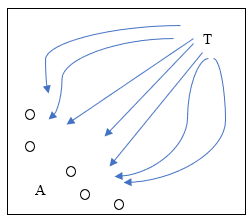
\includegraphics[width=0.5\textwidth]{p3_2.png}
  \caption{Possibilities for shortest paths from the target to the agent in Repeated Backward A*}
\end{figure}

Since the agent explores many more paths in Repeated Backward A* than in Repeated Forward A*, the agent spends more time to examine those paths. As a result, Repeated Backward A* is usually slower than Repeated Forward A*.

%----------------------------------------------------------------------------------------
%	SECTION 5
%----------------------------------------------------------------------------------------

\section{Part 4 - Heuristics in the Adaptive A*}

\subsection{Prove that “the Manhattan distances are consistent in gridworlds in which the agent can move only in the four main compass directions.”}
For a node n, a neighbor $n_0$, and action a, the definition of consistency is \[ \forall (n,a,n_0): h(n) \leq  c(n,a,n_0)+h(n_0)\]

Show that this is true, given that the h-value is the Manhattan distance, and the agent can move only in the four main compass directions.\\

Let the coordinates of n to be $(x_n,y_n)$.\\
Let the coordinates of $n_0$ to be $(x_{n_0},y_{n_0})$.\\
Let the coordinates of the goal, g, to be $(x_g,y_g)$.\\

By the definition of the heuristic function,
\[ h(n)=|x_g-x_n|+|y_g-y_n|)\]
\[ h(n_0)=|x_g-x_{n_0}|+|y_g-y_{n_0}|)\]

Also, since the agent can move only in the four main compass directions
\[ c(n,a,n_0)\geq|x_{n_0}-x_n|+|y_{n_0}-y_n|)\]

Next, the following are true because of $|x+y|\leq|x|+|y|$
\[ |x_g-x_{n_0}+x_{n_0}-x_n|=|x_g-x_n|\leq|x_g-x_{n_0}|+|x_{n_0}-x_n| \]
\[ |y_g-y_{n_0}+y_{n_0}-y_n|=|y_g-y_n|\leq|y_g-y_{n_0}|+|y_{n_0}-y_n| \]

Therefore, by adding the above inequalities together,
\[ h(n)=|x_g-x_n|+|y_g-y_n|\leq|x_g-x_{n_0}|+|y_g-y_{n_0}|+|x_{n_0}-x_n|+|y_{n_0}-y_n| \]

Which, by definition, means
\[h(n)\leq c(n,a,n_0)+h(n_0) \] 

Since n may be any node and $n_0$ may be any neighbor of n, the Manhattan distances are consistent in gridwords in which the agent can move only in the four main compass directions.

\[ \forall (n,a,n_0): h(n) \leq  c(n,a,n_0)+h(n_0)\]

\subsection{Prove that Adaptive A* leaves initially consistent h-values consistent even if action costs can increase.}

For a node n, a neighbor $n_0$, and action a, the definition of consistency is \[ \forall (n,a,n_0): h(n) \leq  c(n,a,n_0)+h(n_0)\]

To show that this is true for Adaptive A*, first, prove that the g-value of the goal is greater than the g-value of any node in the closed list. We will use the claim from the first proof to prove that the h-values are consistent.

\begin{itemize}
	\item Proof 1. Prove that $g(goal) \geq g(n) $ . Let goal be the goal state and let n be any node that is in the closed list before reaching that goal state.\\
	
	We know that n is any node in the closed list. Let n' be the next node after n has been explored that is on the optimal path from the start state to the goal state, as shown in Figure 6.

	\begin{figure}[h!]
  		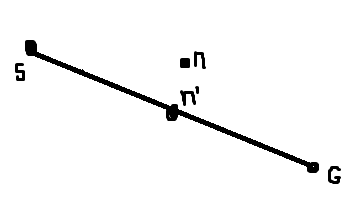
\includegraphics[width=0.5\textwidth]{p4_0.png}
 		 \caption{Illustration of n and n' . Let the black line be the optimal path from the start to the goal state.}
	\end{figure}

	The f-value of n is less than or equal to the f-value of n' since we assume n to be in the closed list before n' was added to it. Therefore,
	\[ g(n)+h(n) \leq g(n')+h(n') \]
	 Also, we know that the f-value of the node n' is less than or equal to the f-value of the goal, by definition of the A* algorithm. Further, the f-value of the goal is the same as the g-value of the goal, since the h-value of the goal is 0. Therefore, 
	\[g(n') +h(n') \leq f(goal)=g(goal) \]
	Putting the inequalities together, 
	\[g(n)+h(n) \leq g(goal) \]
	\[g(n) \leq g(goal) \]

	\item Proof 2. Use the claim from proof 1 to prove that the h-values from the Adaptive A* algorithm are consistent, that $ \forall (n,a,n_0): h(n) \leq  c(n,a,n_0)+h(n_0)$
	
	Let n be a node, $n_0$ be a neighbor of node n, and a be an action.
	By the definition of the heuristic function for adaptive A*, 
	\[h(n)=g(goal)-g(n) \]
	\[h(n_0)=g(goal)-g(n_0) \]
	Because of proof 1, which proves that difference between g-value of the goal and the g-value of any node in the closed list is always positive
	\[h(n)=|g(goal)-g(n)| \]
	\[h(n_0)=|g(goal)-g(n_0)| \]
	Since n is a neighbor of $n_0$ ,
	\[c(n,a,n_0)=|g(n_0)-g(n)|=1 \]
	The following is true because of $|x+y|\leq|x|+|y|$
	\[|g(goal)-g(n_0)+g(n_0)-g(n)| \leq |g(goal)-g(n_0)|+|g(n_0)-g(n)| \]
	Therefore, 
	\[ h(n)= |g(goal)-g(n)| = |g(goal)-g(n_0)+g(n_0)-g(n)|  \]
	\[ \leq |g(goal)-g(n_0)|+|g(n_0)-g(n)|=h(n_0)+c(n,a,n_0) \]
	Since n may be any node and $n_0$ may be any neighbor of n, heuristics are consistent in the Adaptive A* algorithm.
	\[ \forall (n,a,n_0): h(n) \leq  c(n,a,n_0)+h(n_0)\]

\end{itemize}




%----------------------------------------------------------------------------------------
%	SECTION 5
%----------------------------------------------------------------------------------------

\section{Part 5 - Heuristics in the Adaptive A*}

\subsection{ Implement and compare Repeated Forward A* and Adaptive A* with respect to their runtime.}

PUT TABLE HERE

\subsection{Explain your observations in detail, that is, explain what you observed and give a reason for the observation.}
Adaptive A* will be faster than Repeated Forward A*. \\

By definition, the heuristic function is the distance from the current state to the goal state. The h-value in the adaptive A* algorithm is always equal to or greater than the h-value in the Repeated Forward A* algorithm, which is always the Manhattan distance.  \\

However, the heuristic function in Adaptive A* is admissible. Therefore, the h-value of a node is always less than the actual shortest distance from the node to the goal state.\\

Since the h-value in Adaptive A* is greater than or equal to that of Repeated Forward A*, it is more accurate than that of Repeated Forward A*. \\

As a result, the f-values of some nodes, whose path to the goal is long due to many blocked cells, will be higher, and those nodes will be correctly less likely to be expanded from the open list.\\


%----------------------------------------------------------------------------------------
%	SECTION 5
%----------------------------------------------------------------------------------------

\section{Part 6 - Memory Issues}

\subsection{Suggest additional ways to reduce the memory consumption of your implementations further.}
x
\subsection{Calculate the amount of memory that they need to operate on gridworlds of size 1001 x 1001 and the largest gridworld that they can operate on within a memory limit of 4 MBytes.}
x




\end{document}